\documentclass[12pt, a4paper]{article}

% --- Packages ---
\usepackage[utf8]{inputenc}
\usepackage{graphicx}
\usepackage{amsmath}
\usepackage{amssymb}
\usepackage{booktabs}
\usepackage{geometry}
\geometry{a4paper, margin=1in}
\usepackage{hyperref}
\usepackage{xcolor}

\title{R\&D on millikelvin-precision temperature sensing with FBG fibers for cryogenic environments}

\author{Jesús Álvarez, Sara Benítez, Jordi Capó, Anselmo Cervera,\\ Victoria García, Simón Teruel, Nadia Yahlali ... \\ \textit{IFIC - CSIC - Universitat de València}}
\date{\today}

\begin{document}

\maketitle

\tableofcontents

\begin{abstract}
Precise temperature monitoring, at the level of a few millikelvin, is essential for the operation of large-scale cryostats equipped with recirculation systems. In particular, the performance of Liquid Argon Time Projection Chambers (LArTPCs), such as those planned for the DUNE experiment, strongly depends on efficient argon purification and mixing, which can be characterized through a sufficiently dense grid of high-precision temperature sensors.
In environments where the use of conventional electrical sensors, such as Resistance Temperature Detectors (RTDs), may be limited by the presence of high electric fields, Fiber Bragg Grating (FBG) sensors provide an attractive alternative. FBGs offer electrical insulation, immunity to electromagnetic interference, and the possibility of multiplexing multiple sensors along a single optical fiber, making them particularly suitable for large cryogenic systems.
In this article, we present the principles and experimental validation of a temperature monitoring system based on an array of FBG sensors, with particular emphasis on the techniques required to achieve millikelvin-level temperature precision. The results demonstrate the potential of FBG arrays for high-precision temperature monitoring in large-scale cryogenic systems.
\end{abstract}

% ==========================================
\section{Introduction (Anselmo)}
% ==========================================

\begin{itemize}
    \item Interest of precise temperature measurements in cryogenic environments
    \item The DUNE example
    \item Motivation for the use of fibers in DUNE
\end{itemize}

% ==========================================
\section{Cryogenic sensing with FBGs}
\label{sec:fbgs}
% ==========================================

\subsection{Sensitivity influencing factors} 
\label{subsec:sensitivity}

At ambient temperature ($300~\text{K}$), the wavelength shift of a bare silica FBG is governed almost entirely by the thermo-optic effect of fused silica ($dn/dT \approx 8.6 \times 10^{-6}~\text{K}^{-1}$), which accounts for over 90\% of the standard $\sim$10~pm/K sensitivity, while thermal expansion contributes negligibly ($\alpha_{\text{silica}} \approx 0.5 \times 10^{-6}~\text{K}^{-1}$). In cryogenic conditions ($77$--$93~\text{K}$), however, the thermo-optic coefficient drops by nearly an order of magnitude (down to $<1.0 \times 10^{-6}~\text{K}^{-1}$) and the thermal expansion of silica becomes negligible ($\alpha_{\text{silica}} < 0.2 \times 10^{-6}~\text{K}^{-1}$), causing the intrinsic sensitivity of bare silica gratings to collapse to less than $1.5~\text{pm/K}$~\cite{Lupi2008,Salin2008,Rajan2013}. To recover high thermal responsivity in cryogenic noble liquid detectors, the optical fiber is functionalized with a polymeric coating that serves as a mechanical thermal transducer:
\begin{equation}
    \frac{\Delta \lambda_B}{\lambda_B} = (\alpha_{\text{silica}} + \zeta) \Delta T + (1 - p_e) \epsilon_z,
    \label{eq:fbg_coating_strain}
\end{equation}
where $\zeta = (1/n)(dn/dT)$ is the normalized thermo-optic coefficient, $p_e \approx 0.22$ is the effective photoelastic constant, and $\epsilon_z$ is the total longitudinal strain in the silica core. Under tension-free mounting the axial strain is purely thermally driven by the differential contraction between the polymer jacket and the glass: $\epsilon_z = \eta (\alpha_{\text{coating}} - \alpha_{\text{silica}}) \Delta T$, where $\eta \le 1$ represents the interfacial strain-transfer efficiency. Because polymer materials maintain cryogenic thermal expansion coefficients orders of magnitude higher than silica ($\alpha_{\text{coating}} \sim 15$--$35 \times 10^{-6}~\text{K}^{-1}$ at $77~\text{K}$, as summarized in Table~\ref{tab:material_cte}), the contracting jacket exerts a strong axial compressive strain on the fiber core, enhancing the cryogenic thermal sensitivity up to $15$--$35~\text{pm/K}$~\cite{Lupi2008,Zhao2007,Rajan2013}.

\begin{table}[htpb]
    \centering
    \footnotesize
    \setlength{\tabcolsep}{4.5pt}
    \caption{Thermal expansion properties and integrated cryogenic contraction of the optical fiber constituents.}
    \label{tab:material_cte}
    \begin{tabular}{lcccc}
        \toprule
        \textbf{Material} & $\boldsymbol{\alpha_{300\,\text{K}}}$ & $\boldsymbol{\alpha_{77\,\text{K}}}$ & $\boldsymbol{\Delta L/L}$ & \textbf{Structural Role} \\
                          & ($10^{-6}\,\text{K}^{-1}$)           & ($10^{-6}\,\text{K}^{-1}$)          & ($300\to 77\,\text{K}$)   &                          \\
        \midrule
        Fused silica        & $\sim 0.5$    & $< 0.2$   & $\sim 0.01\%$       & Core / Cladding glass~\cite{NIST_CryoMaterials} \\
        Polyimide           & $30$--$40$    & $12$--$20$ & $\sim 0.4$--$0.6\%$ & Primary buffer coating~\cite{Zhao2007,NIST_CryoMaterials} \\
        PEEK                & $45$--$50$    & $20$--$30$ & $\sim 1.0$--$1.2\%$ & Thermoplastic jacket~\cite{NIST_CryoMaterials} \\
        Ormocer / Ormocer-T & $100$--$130$  & $25$--$40$ & $\sim 1.2$--$1.5\%$ & Hybrid optical polymer~\cite{Popall1998} \\
        \bottomrule
    \end{tabular}
\end{table}

The magnitude of the strain transferred to the fiber core depends fundamentally on the cross-sectional area ratio between the jacket and the glass, $A_{\text{coating}}/A_{\text{glass}} = (D^2 - d^2)/d^2$ (where $d = 125~\mu\text{m}$ is the cladding diameter and $D$ is the outer coating diameter), as well as the elastic modulus and interfacial adhesion of the polymer~\cite{Bock2004,Zhao2007}. Consequently, increasing the coating thickness from a standard thin layer ($D \approx 200~\mu\text{m}$, $A_{\text{coating}}/A_{\text{glass}} \approx 1.56$) to an extruded thick jacket ($D \approx 440$--$450~\mu\text{m}$, $A_{\text{coating}}/A_{\text{glass}} \approx 11.5$) markedly amplifies the mechanical force exerted on the grating, providing a systematic handle to study the trade-off between thermal responsivity, mechanical stiffness, and response time.

\subsection{FBGs and coatings tested}
\label{subsec:fibers}

For deployment in large-scale noble liquid time projection chambers such as DUNE, coating selection is constrained by strict chemical purity and cryogenic resilience. Polymers must exhibit negligible outgassing of electronegative contaminants (such as $\text{O}_2$ and $\text{H}_2\text{O}$) to prevent the attenuation of drifting ionization electrons~\cite{Acciarri2020ProtoDUNE}, while maintaining high mechanical adhesion to prevent micro-cracking or delamination under rapid thermal cycles between $300~\text{K}$ and $77~\text{K}$. To evaluate these criteria, five commercial fiber configurations encompassing three representative coating classes were characterized:
\begin{itemize}
    \item \textbf{Ormocer and Ormocer-T:} Organic-inorganic hybrid optical polymers (developed by Fraunhofer-ISC and commercialized by FBGS) combining inorganic polysiloxane networks with cross-linked organic side chains, offering strong chemical bonding to silica and elevated thermal durability~\cite{Popall1998}.
    \item \textbf{Polyimide:} High-temperature aromatic polymer (ENGIONIC) widely recognized for its high radiation hardness, vacuum compatibility, and low outgassing, extensively used in aerospace and cryogenic instrumentation~\cite{Zhao2007}.
    \item \textbf{PEEK:} Polyether ether ketone (ENGIONIC), an advanced semi-crystalline thermoplastic with high mechanical strength, tested in both thin-jacket ($200~\mu\text{m}$) and thick-jacket ($440$--$450~\mu\text{m}$) geometries to isolate the structural influence of coating volume~\cite{NIST_CryoMaterials,Rajan2013}.
\end{itemize}

The technical specifications of the characterized fiber samples, along with their nominal dimensions, grating count, and suppliers, are summarized in Table~\ref{tab:fiber_specs}.

\begin{table}[htpb]
    \centering
    \scriptsize
    \setlength{\tabcolsep}{4pt}
    \caption{Technical specifications of the characterized optical fibers and polymer coatings tested across the $77$--$93~\text{K}$ cryogenic calibration campaign.}
    \label{tab:fiber_specs}
    \begin{tabular}{llccccc}
        \toprule
        \textbf{Fiber ID} & \textbf{Coating Material} & \textbf{Coating} & \textbf{Cladding} & \textbf{FBGs Total} & \textbf{FBG Length} & \textbf{Supplier} \\
                          &                            & ($\mu\text{m}$)  & ($\mu\text{m}$)   & (In Cryo)           & (mm)                &                   \\
        \midrule
        DW-3              & Ormocer-T                  & 200              & 125               & 5 (4)               & 10                  & FBGS              \\
        FBGS-2            & Ormocer                    & 200              & 125               & 4 (4)               & 8                   & FBGS              \\
        PEEK-3            & PEEK                       & 200              & 125               & 1 (1)               & 5                   & ENGIONIC          \\
        POLY-2            & Polyimide                  & 200              & 125               & 4 (2)               & 9                   & ENGIONIC          \\
        PEEK-4            & PEEK (Thick jacket)        & 440--450         & 125               & 3 (2)               & 5                   & ENGIONIC          \\
        PEEK-7            & PEEK (Thick jacket)        & 410--420         & 125               & 3 (2)               & 5                   & ENGIONIC          \\
        \bottomrule
    \end{tabular}
\end{table}

% ==========================================
\section{FBGs testing methods}
\label{sec:setup}
% ==========================================

\subsection{Experimental Setup}
\label{subsec:setup}

The experimental setup used for the thermal characterization of FBG fibers is schematically shown in Fig.~\ref{fig:setup}. It consists of four main elements: the pressurized vessel, the gas line, the sensing assembly, and the readout instrumentation.

The cryostat vessel has a non-uniform cylindrical geometry, consisting of an expanded lower reservoir (\textcolor{red}{approx. XX~mm outer diameter, XX~mm height?}) that accommodates the bulk liquid nitrogen bath and the immersed sensing capsule, surmounted by a narrower neck section (\textcolor{red}{approx. XX~mm diameter?}) and capped with an upper CF-40 cross assembly. The vessel ports are arranged across two vertical levels. At the lower neck level, two lateral ports provide access for pressure logging and the internal diagnostic RTD array used to track the liquid nitrogen level. The top flange of the CF-40 cross---opened for capsule insertion---is hermetically sealed using an OFHC copper gasket tightened in three progressive torque stages (8, 12, and $14~\text{N}\cdot\text{m}$) to guarantee vacuum-tight containment up to $5~\text{bar}$. This top cross incorporates two lateral CF-40 flanges: one equipped with hermetic optical feedthroughs (supporting up to two fibers) routed to the FAZT I4-16 interrogator, and the opposite one providing the dedicated electrical feedthrough for the two reference RTDs housed inside the sensing capsule alongside the fiber.

The sensing assembly consists of a cylindrical 3D-printed support (\textcolor{red}{approx. XX~mm diameter?}), where two calibrated reference RTDs fit into diametrically opposed slots. The optical fiber is wound around the outer perimeter of the cylinder directly over the RTD locations, with the fiber end softly secured via a Teflon clamp to prevent slipping. The sensing assembly is housed within a protective aluminum capsule that acts as a thermal buffer to moderate cooling rates and prevent direct hydrodynamic disturbances on the fiber gratings during boiling. The entire capsule is mounted at the bottom of a long stainless steel insertion rod that guides the internal optical patch cord (coupled to the test fiber) and the RTD wiring to the top flanges.

The cryostat is connected to a dedicated gas handling line. A digital pressure transmitter with a local digital display is mounted on one of the lower neck ports and interfaced to an Arduino acquisition board for continuous computer logging. An exhaust gas line equipped with a manual fine-metering needle valve allows fine regulation of the boil-off gas release to depressurize the vessel in controlled steps.

The data acquisition system consists of two independent modules, one for optical signal interrogation and one for thermal monitoring, synchronized through a post-acquisition time-stamping procedure. The optical sensors are interrogated using a FAZT I4-16 optical interrogator (Femto Sensing International). The instrument provides 16 optical channels and supports up to 30 FBG sensors per channel, operating over the $1529$--$1568.2~\text{nm}$ wavelength range with a wavelength resolution of $1~\text{pm}$, an absolute accuracy below $1~\text{pm}$, and an acquisition frequency of $200~\text{Hz}$~\cite{FemtoSenseManual}. The reference RTD sensors are read out using a dedicated electronic system developed at CERN, providing a stable $1~\text{mA}$ current source for sensor excitation and a multiplexing circuit acquiring signals from up to 24 channels. The voltage measurements are performed using a National Instruments CompactRIO-FPGA equipped with a 24-bit NI-9238 analogue input module, converting platinum resistance to temperature via the Callendar--Van Dusen equation with a measurement repeatability better than $0.5~\text{mK}$~\cite{RTDs_paper}. The technical specifications of the DAQ and interrogation hardware are summarized in Table~\ref{tab:daq_specs}.

\begin{figure}[htpb]
    \centering
    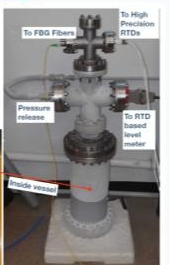
\includegraphics[width=0.95\textwidth]{figures/pressure_setup.png}
    \caption{Schematic of the pressure-based experimental setup used for cryogenic FBG characterization, showing the pressurized vessel with liquid nitrogen, internal sensing capsule, gas handling line with fine-metering valve, and independent optical and thermal readout instrumentation.}
    \label{fig:setup}
\end{figure}

\begin{table}[htpb]
    \centering
    \caption{Technical specifications of the DAQ and optical interrogation hardware.}
    \label{tab:daq_specs}
    \begin{tabular}{lcc}
        \toprule
        \textbf{Parameter} & \textbf{Optical Interrogator} & \textbf{RTD Readout (DAQ)} \\
        \midrule
        Model & FAZT I4-16 & CERN CompactRIO NI-9238 \\
        Sampling Rate & 200 Hz & 10 Hz \\
        Resolution & 1 pm (30 fm relative) & $\leq 0.5\,\mathrm{mK}$ \\
        Interface & Ethernet & NI-DAQmx \\
        Accuracy & $< 1\,\mathrm{pm}$ & $< 2.5\,\mathrm{mK}$ \\
        \bottomrule
    \end{tabular}
\end{table}

\subsection{Operating protocol}
\label{subsec:protocol}

The calibration uses the saturation temperature of liquid nitrogen under controlled pressure, avoiding the need for active electrical heaters. The procedure follows five steps:

\begin{enumerate}
    \item \textbf{Cooling and filling:} Liquid nitrogen is transferred into the vessel until the internal level-diagnostic RTD array is submerged. An open pre-cooling period ($\sim$40~minutes) allows the vessel mass to cool down and boiling turbulence to subside.
    %\item \textbf{Capsule insertion:} The sensing capsule---housing the 3D-printed support with the test fiber and the two reference RTDs---is lowered progressively into the liquid nitrogen bath in discrete stages using mechanical spacers to mitigate thermal shock. At its final position near the bottom of the vessel, the entire capsule is completely submerged in the liquid.
    \item \textbf{Capsule insertion and cooldown:} The sensing capsule---housing the 3D-printed support with the test fiber and the two reference RTDs---is lowered into the cryostat using mechanical spacers. The top opening of the capsule is initially held above the liquid nitrogen level until the internal RTDs drop below 85~K, minimizing thermal shock before liquid enters the capsule. Once cooled, the capsule is fully lowered to the bottom of the vessel, completely submerged in the liquid bath. The top opening of the capsule is initially held above the liquid nitrogen level until the internal RTDs drop below 85~K, minimizing thermal shock before liquid enters the capsule. Once cooled, the capsule is fully lowered to the bottom of the vessel, completely submerged in the liquid bath.
    \item \textbf{Vessel sealing:} The top CF-40 flange is sealed with the copper gasket. The fibers are connected to the interrogator and the RTDs to the DAQ system.
    \item \textbf{High-pressure stabilization:} With the exhaust valve closed, natural nitrogen boil-off raises the vessel pressure to 3.0--4.0~bar. The cryostat is left for 1.0--1.5~hours until ambient heat leak warms the liquid and the sensors reach a stable temperature plateau (90--93~K), confirming thermodynamic equilibrium.
    \item \textbf{Stepped depressurization:} The pressure is then decreased in steps of 0.3--0.5~bar using the manual needle valve down to atmospheric pressure ($\sim$1~bar). After each step, the pressure is held constant for several minutes to allow the bath to stabilize at the new boiling temperature.
\end{enumerate}

The liquid level is tracked throughout the run using the vertical RTD array to ensure the capsule remains immersed. Each fiber was tested in three independent runs on different days, warming the vessel to room temperature between runs to evaluate thermal cycling repeatability ($300~\text{K} \leftrightarrow 77~\text{K}$).

To verify that the bath reached saturation equilibrium during the plateaus, we compared the measured $(P, T)$ points with the theoretical nitrogen saturation curve from NIST~\cite{Lemmon2025NIST,Edejer1967}:
\begin{equation}
    \log_{10}(P_{\text{abs}}/\text{bar}) = A - \frac{B}{T + C},
    \label{eq:antoine}
\end{equation}
with NIST coefficients $A = 3.7362$, $B = 264.651$, and $C = -6.788~\text{K}$. Figure~\ref{fig:n2_saturation_with_data} shows all 124 plateaus recorded across 18 runs with different fibers over several months. A three-parameter Antoine fit to our data gives $A = 2.9085$, $B = 152.08$, and $C = -25.25~\text{K}$, agreeing with NIST predictions within 0.25~K over the 77--93~K range.

The lower panel of Figure~\ref{fig:n2_saturation_with_data} shows the temperature residuals, $\Delta T = T_{\text{RTD}} - T_{\text{NIST}}(P_{\text{abs}})$. The average residual across all plateaus is $\langle \Delta T \rangle = -0.14~\text{K}$ ($\text{RMSE} = 0.28~\text{K}$), with 80\% of the points within $\pm 0.3~\text{K}$. The small residual spread is consistent with pressure gauge accuracy and local atmospheric variations ($\pm 20~\text{mbar}$). This confirms that the nitrogen bath was at saturation and validates the RTD temperature as a reliable reference.

\begin{figure}[htpb]
    \centering
    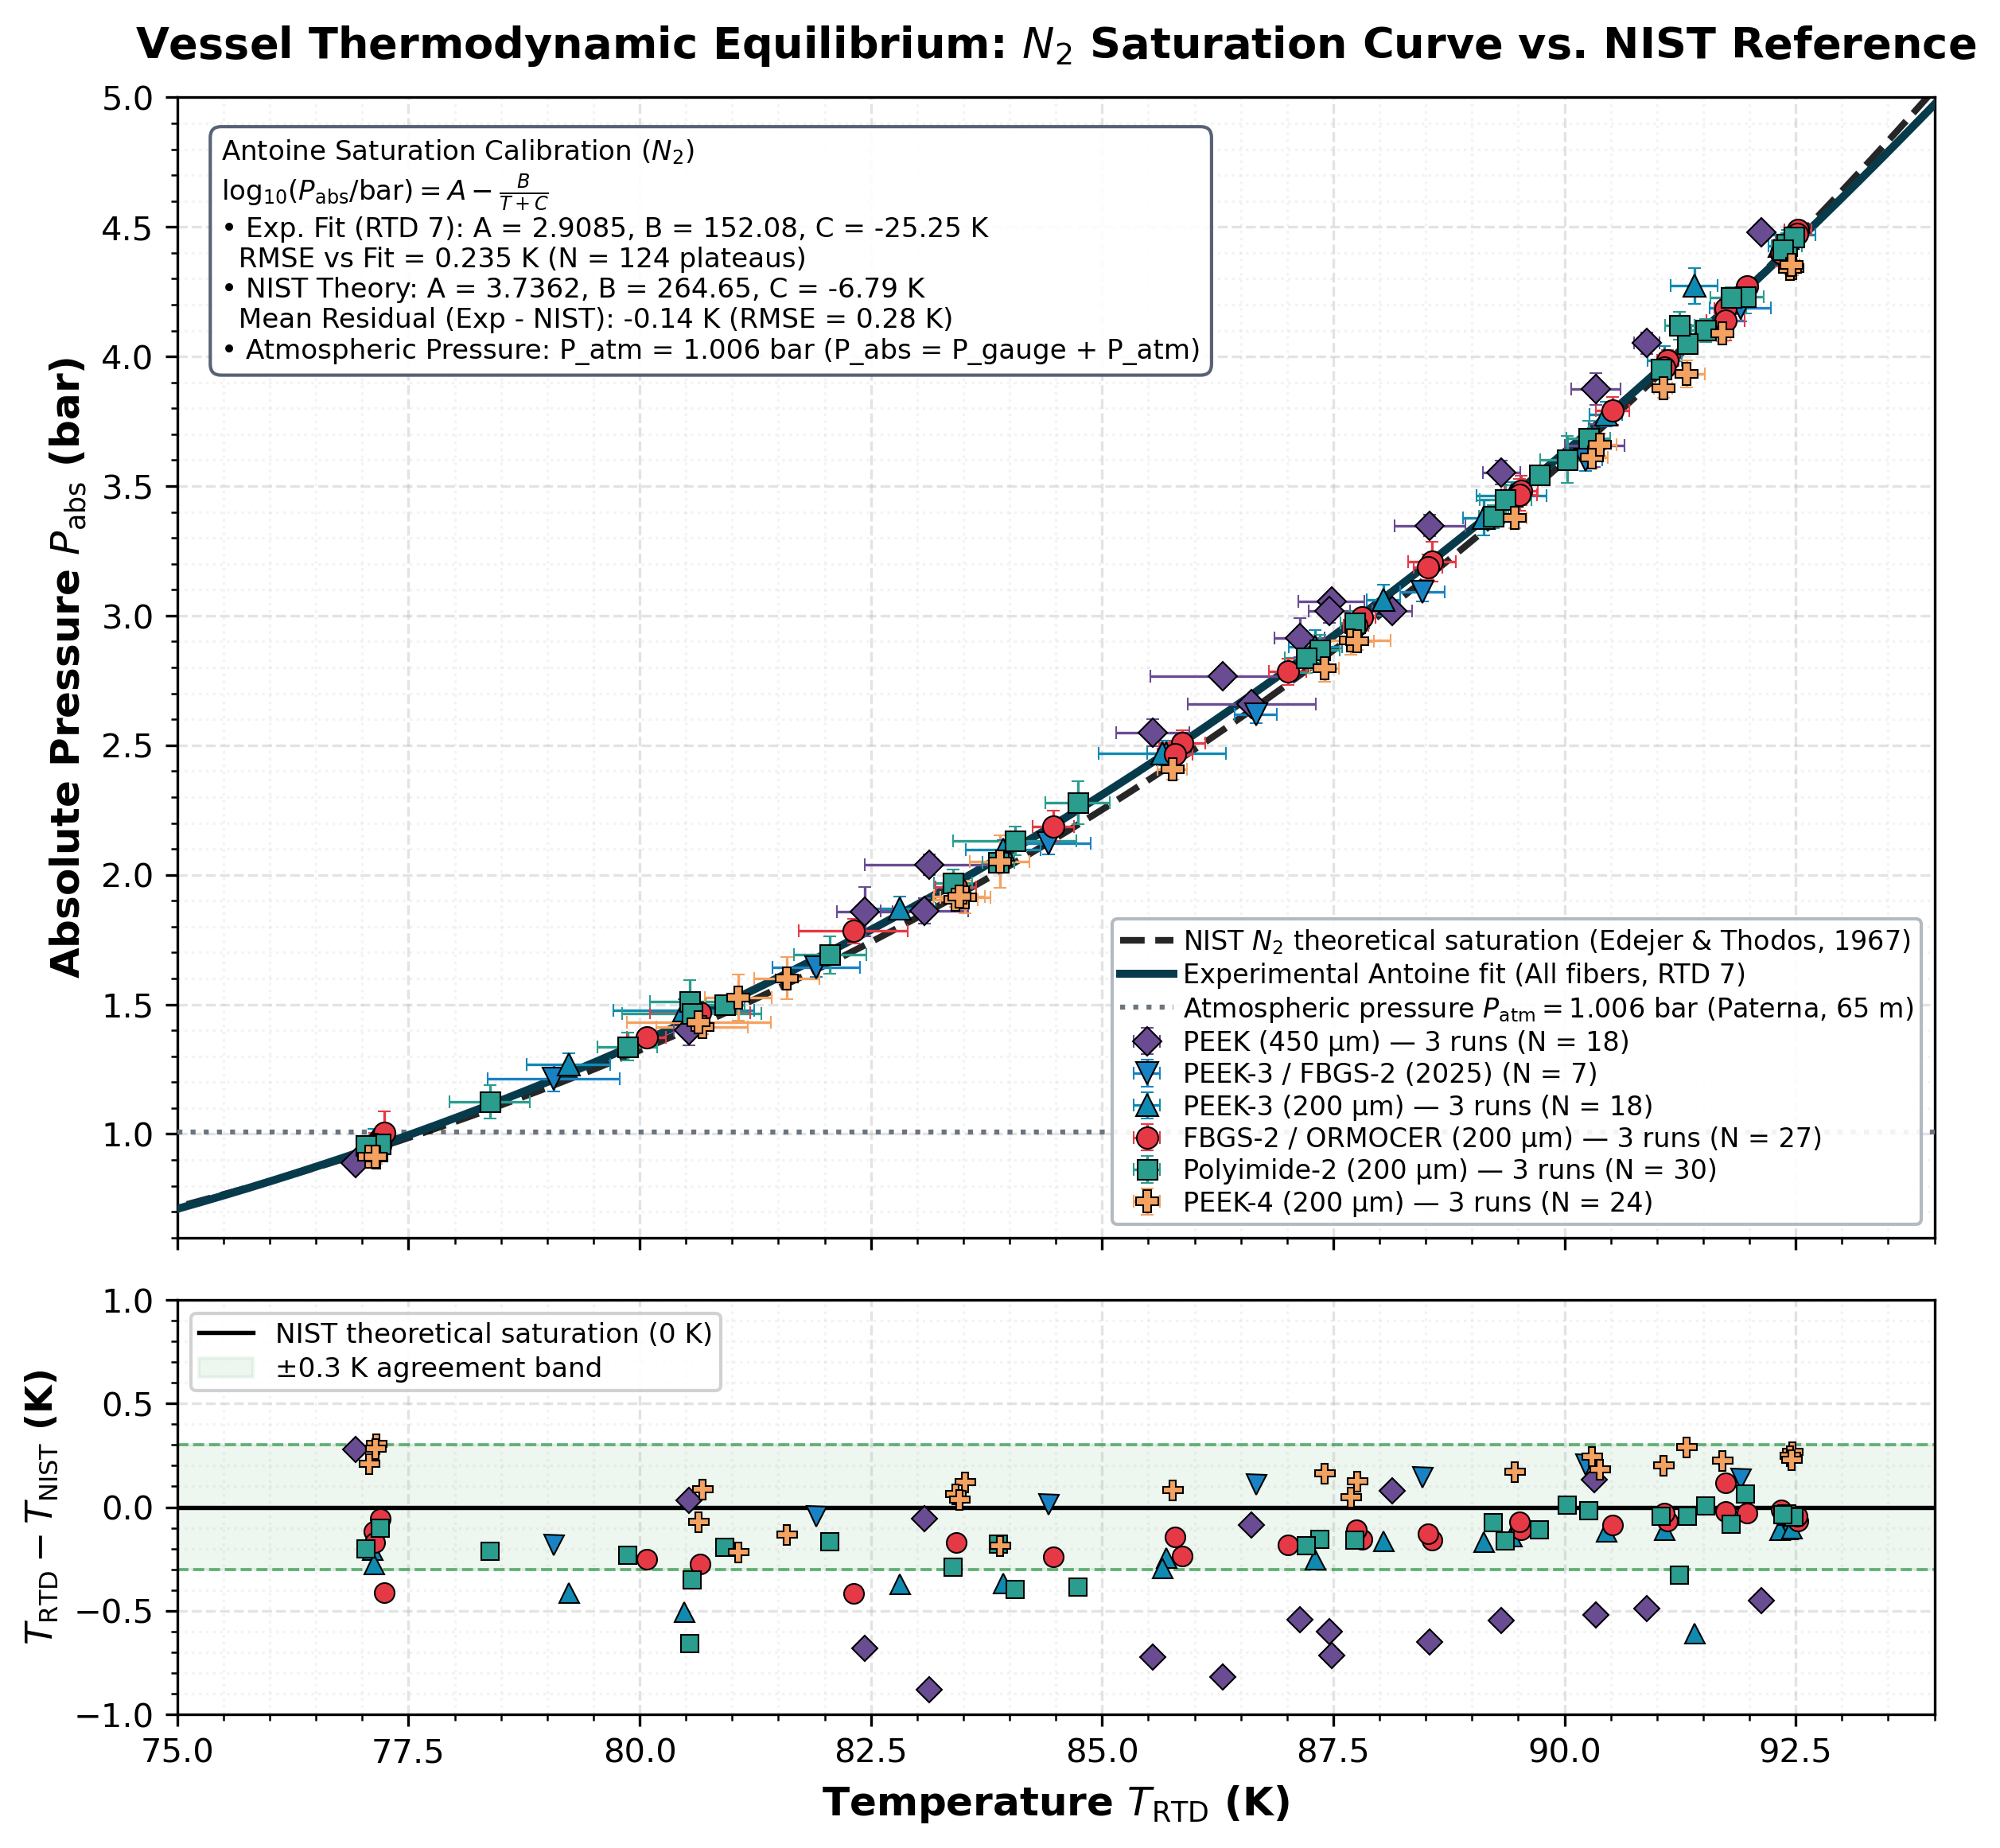
\includegraphics[width=0.88\textwidth]{figures/n2_saturation_all_fibers2.png}
    \caption{Thermodynamic equilibrium validation of the cryogenic vessel. Top panel: Measured absolute pressure $P_{\text{abs}}$ as a function of capsule RTD temperature $T_{\text{RTD}}$ for all 124 plateaus. Solid line: experimental Antoine fit; dashed line: NIST reference curve~\cite{Lemmon2025NIST,Edejer1967}. Bottom panel: Temperature residuals $T_{\text{RTD}} - T_{\text{NIST}}$ relative to NIST, showing agreement within $\pm 0.3~\text{K}$ for 80\% of the points.}
    \label{fig:n2_saturation_with_data}
\end{figure}

\subsection{Analysis procedures}
\label{subsec:analysis_procedure}

The data processing methodology translates the synchronized time series into cryogenic thermal sensitivities while accounting for experimental uncertainties across successive thermal cycles. The procedure follows five sequential steps, illustrated in Figure~\ref{fig:data_workflow}:

\begin{enumerate}
    \item \textbf{Temporal alignment and synchronisation:}
    Continuous measurements from the optical interrogator, the RTD readout system, and the digital pressure sensor are referenced to a common global time scale. Absolute UTC timestamps are used to correct clock offsets between the acquisition systems. Because each instrument operates at a different sampling rate (200~Hz for the optical interrogator and 10~Hz for the RTD readout), all time series are aligned on this shared temporal reference, allowing temperature, pressure, and Bragg wavelength to be directly correlated throughout the entire cooldown run.

    \item \textbf{Plateau selection and duration standardisation:}
    Following each depressurisation step, the time series are inspected to identify steady-state equilibrium intervals, as shown in Figure~\ref{fig:data_workflow}(a). The initial transient phase immediately following valve adjustment---characterised by bulk boiling and rapid temperature drop---is excluded. Stable plateau windows are selected within the flat region of each pressure step, ensuring that both the initial thermal relaxation and the edge preceding the subsequent pressure decrease are avoided. To prevent longer intervals from having a disproportionate weight in the linear regression, all plateau windows within a given run are standardized to an identical duration ($\Delta t$), matching the shortest stable period identified during that cycle (typically between $5$ and $11~\text{minutes}$; $\Delta t = 9.0~\text{minutes}$ in Figure~\ref{fig:data_workflow}(a)). This ensures that every calibration point represents the same sample size ($N$) and integration time.

    \item \textbf{Plateau averaging and polarization handling:}
    For each optical sensor, the effective wavelength trace is obtained by averaging the two orthogonal polarization modes, $\lambda_B(t) = (\lambda_{B,P}(t) + \lambda_{B,S}(t))/2$, which cancels out peak shifts induced by fiber birefringence. Within each standardized plateau window, the mean temperature and Bragg wavelength values ($\mu_T, \mu_\lambda$) are computed. The uncertainty associated with each plateau mean is evaluated using the Standard Error of the Mean ($\text{SEM} = \sigma / \sqrt{N}$), as illustrated in the plateau zoom of Figure~\ref{fig:data_workflow}(b). Given the large number of acquired samples ($N \sim 10^4$--$10^5$ points per plateau at 200~Hz), random instrumentation noise is strongly suppressed, resulting in sub-millikelvin and sub-picometer statistical uncertainties for the plateau means.

    \item \textbf{Thermal sensitivity extraction:}
    The thermal sensitivity is determined by performing a linear least-squares regression on the plateau-averaged points, as shown in Figure~\ref{fig:data_workflow}(c):
    \begin{equation}
        \lambda_B(T) = \lambda_0 + S \cdot (T - T_0),
        \label{eq:linear_sensitivity}
    \end{equation}
    where the slope $S = \mathrm{d}\lambda_B/\mathrm{d}T$ ($\text{pm/K}$) represents the experimental sensitivity, and $\sigma_{\text{fit}}$ is the fit uncertainty.
    
    This measured slope corresponds directly to the derivative of Eq.~\ref{eq:fbg_coating_strain}. Assuming pure thermal contraction without external mechanical loads ($\epsilon_z = \eta (\alpha_{\text{coating}} - \alpha_{\text{silica}}) \Delta T$), $S$ can be separated into two contributions:
    \begin{equation}
        S = \frac{\Delta \lambda_B}{\Delta T} = \lambda_{B,0} \underbrace{(\alpha_{\text{silica}} + \zeta)}_{S_{\text{bare}}} + \lambda_{B,0} \underbrace{(1 - p_e) \eta (\alpha_{\text{coating}} - \alpha_{\text{silica}})}_{S_{\text{strain}}},
        \label{eq:sensitivity_physics}
    \end{equation}
    where $S_{\text{bare}} \approx \lambda_{B,0} (\alpha_{\text{silica}} + \zeta) < 1.3~\text{pm/K}$ is the small intrinsic contribution from bare silica at cryogenic temperatures, and $S_{\text{strain}}$ is the dominant enhancement provided by the contracting polymer coating, scaled by the strain-transfer efficiency $\eta$.

    \item \textbf{Repeatability and array uniformity:}
    While the fit uncertainty $\sigma_{\text{fit}}$ reflects the statistical scatter within a single measurement, the primary experimental uncertainty arises from the reproducibility between thermal cycles. To quantify this, the calibration was repeated over $R = 3$ independent cooldown runs ($300~\text{K} \leftrightarrow 77~\text{K}$):
    \begin{enumerate}
        \item \textit{Thermal cycling repeatability:} For each sensor $j$, the mean sensitivity across the three runs $\{S_{j,1}, S_{j,2}, S_{j,3}\}$ is calculated as:
        \begin{equation}
            \bar{S}_j = \frac{1}{R} \sum_{r=1}^{R} S_{j,r},
        \end{equation}
        and the run-to-run repeatability is given by the sample standard deviation:
        \begin{equation}
            \sigma_{\text{rep}, j} = \sqrt{\frac{1}{R - 1} \sum_{r=1}^{R} (S_{j,r} - \bar{S}_j)^2}.
            \label{eq:repeatability_error}
        \end{equation}
        
        \item \textit{Fiber array uniformity:} For fibers with $M$ multiplexed sensors, the overall fiber sensitivity is the average across all sensors, $\bar{S}_{\text{fiber}} = \frac{1}{M} \sum_{j=1}^{M} \bar{S}_j$. The inter-sensor standard deviation:
        \begin{equation}
            \sigma_{\text{unif}} = \sqrt{\frac{1}{M - 1} \sum_{j=1}^{M} (\bar{S}_j - \bar{S}_{\text{fiber}})^2}
        \end{equation}
        quantifies the sensitivity variation between sensors along the same fiber.
    \end{enumerate}
\end{enumerate}

\begin{figure}[htpb]
    \centering
    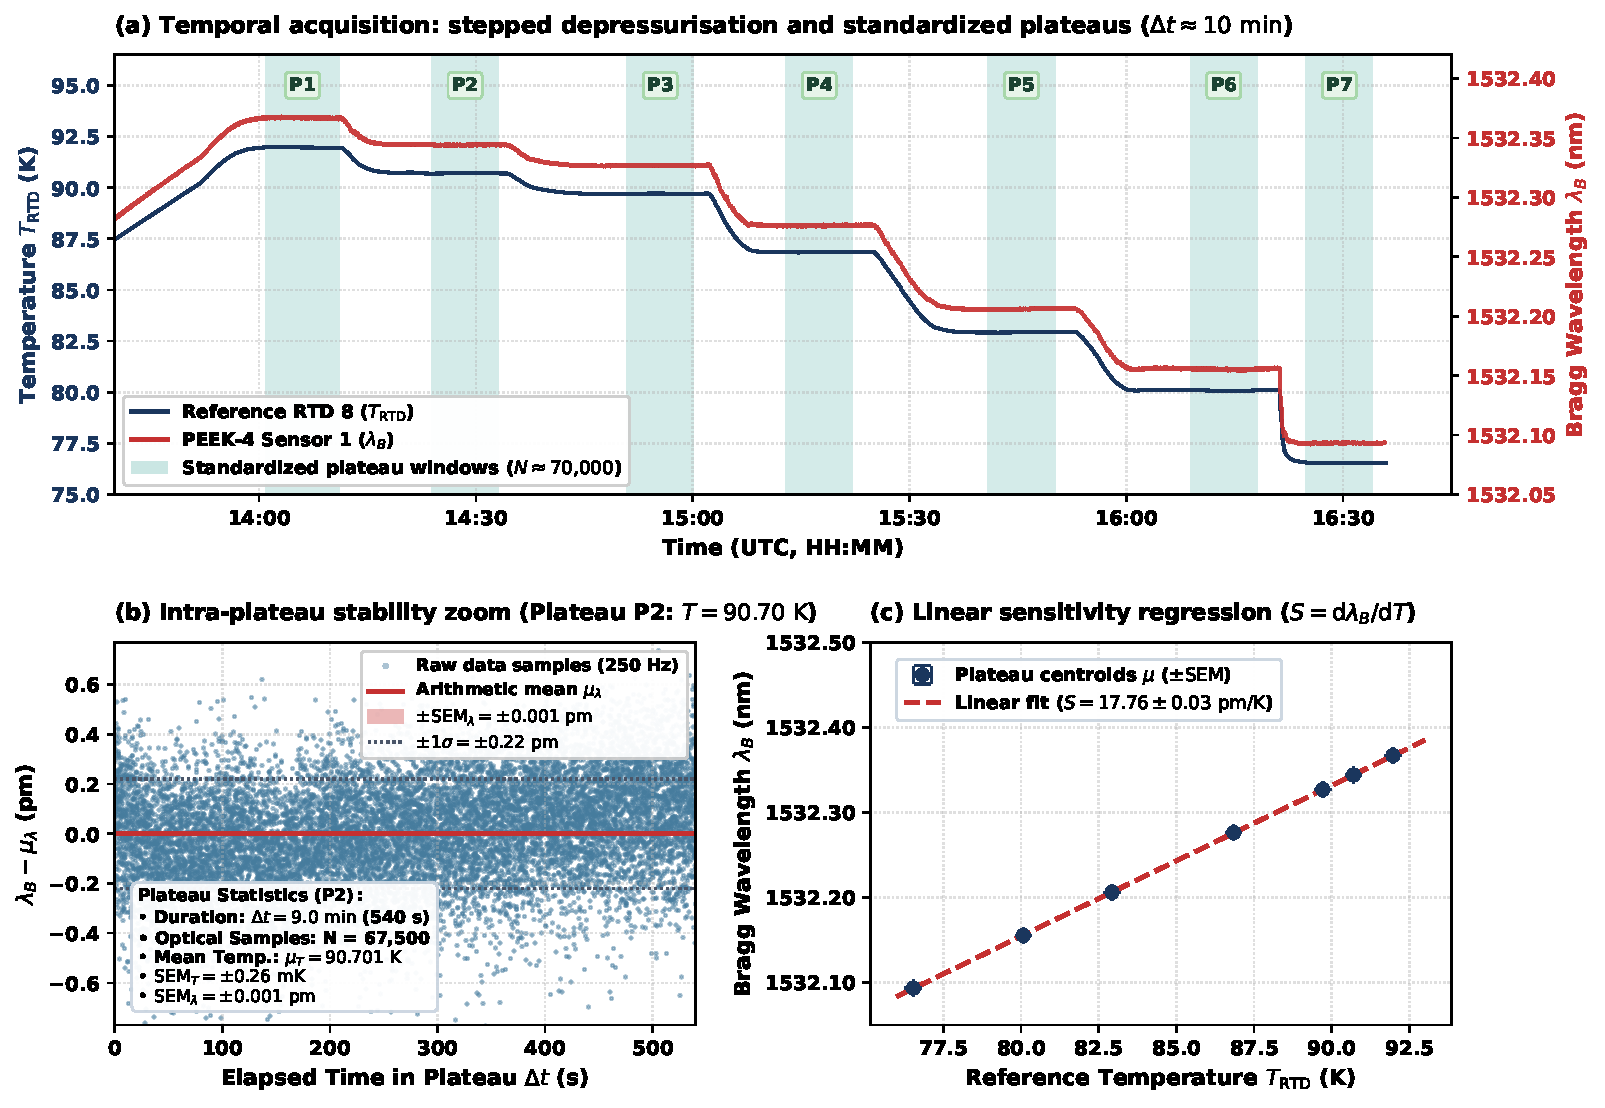
\includegraphics[width=1.0\textwidth]{figures/workflow_diagram.pdf}
    \caption{Key milestones of the data reduction and sensitivity extraction workflow illustrated for Sensor~1 of the PEEK-4 fiber (Run~1, $400\,\mu\text{m}$ coating diameter): (a) Identification of seven steady-state equilibrium plateaus ($P_1$--$P_7$, shaded teal bands) during stepped depressurisation spanning $76.5$--$92.0~\text{K}$, displaying synchronised reference temperature $T_{\text{RTD}}(t)$ (RTD-8 inside the capsule, left axis) and Bragg wavelength $\lambda_B(t)$ (right axis); (b) Zoom-in of representative plateau $P_2$ ($T = 90.70~\text{K}$) over a standardised dwell of $\Delta t = 9.0~\text{min}$ ($N = 67{,}500$ points at $200~\text{Hz}$), showing the stable wavelength trace, plateau mean $\mu_\lambda$, intra-plateau uncertainty band ($\pm\text{SEM}_\lambda = \pm 0.001~\text{pm}$), and raw noise spread ($\pm 1\sigma = \pm 0.22~\text{pm}$); and (c) Final linear least-squares regression applied to the set of plateau means ($\mu_\lambda$ vs. $\mu_T$), yielding the cryogenic thermal sensitivity slope ($S = 17.76 \pm 0.03~\text{pm/K}$, $R^2 = 0.9999$).}
    \label{fig:data_workflow}
\end{figure}

\section{Results and discussion (Vicky)}
\label{sec:results}
% ==========================================

\subsection{Thermal inertia of FBGs vs RTDs (For later ??) (Vicky)}

\begin{itemize}
    \item Observation of thermal lag between optical sensors (FBGs) and electrical sensors (RTDs).
    \item Evaluation of coating thickness impact on thermal response time.
    \item Evaluation of intrinsic hardware and readout latency:.
\end{itemize}

\begin{figure}[htpb]
    \centering
    % \includegraphics[width=0.8\textwidth]{figures/transient_analysis.pdf}
    \vspace{5cm} 
    \caption{Normalized transient response during a pressure step. The temporal shift ($\Delta t$) between the FBG wavelength response and the reference RTD temperature indicates the thermal lag attributed to the coating and ...}
    \label{fig:time_shift_normalized}
\end{figure}

\begin{table}[htpb]
    \centering
    \caption{Measured thermal lag ($\Delta t$) for different fiber coatings during a 1-bar pressure transition.}
    \label{tab:thermal_lag}
    \begin{tabular}{lccc}
        \toprule
        \textbf{Fiber ID} & \textbf{Coating} & \textbf{Diameter ($\mu m$)} & \textbf{Avg. Lag ($\Delta t$, s)} \\
        \midrule
        DW-3 & Ormocer-T & 250 & $? \pm ?$ \\
        PEEK-4 & PEEK & 400 & $? \pm ?$ \\
        PEEK-3 & PEEK & 200 & $? \pm ?$ \\
        POLY-2 & Polyimide & 200 & $? \pm ?$ \\
        \bottomrule
    \end{tabular}
\end{table}

%-------------------------------------------------
\subsection{Temperature Sensitivity of Different Fiber Configurations}
\label{subsec:sensitivity_results}

The cryogenic thermal sensitivity of each optical fiber configuration was characterized across the liquid nitrogen saturation window ($77.3$--$93.5~\text{K}$) by applying the plateau-averaged linear regression protocol established in Section~\ref{subsec:analysis_procedure}. A representative single-run calibration is illustrated in Figure~\ref{fig:control_plot_run1} for the dual-sensor PEEK-4 array ($400~\mu\text{m}$ jacket diameter) during Run~1 (09-06-2026).

\begin{figure}[htpb]
    \centering
    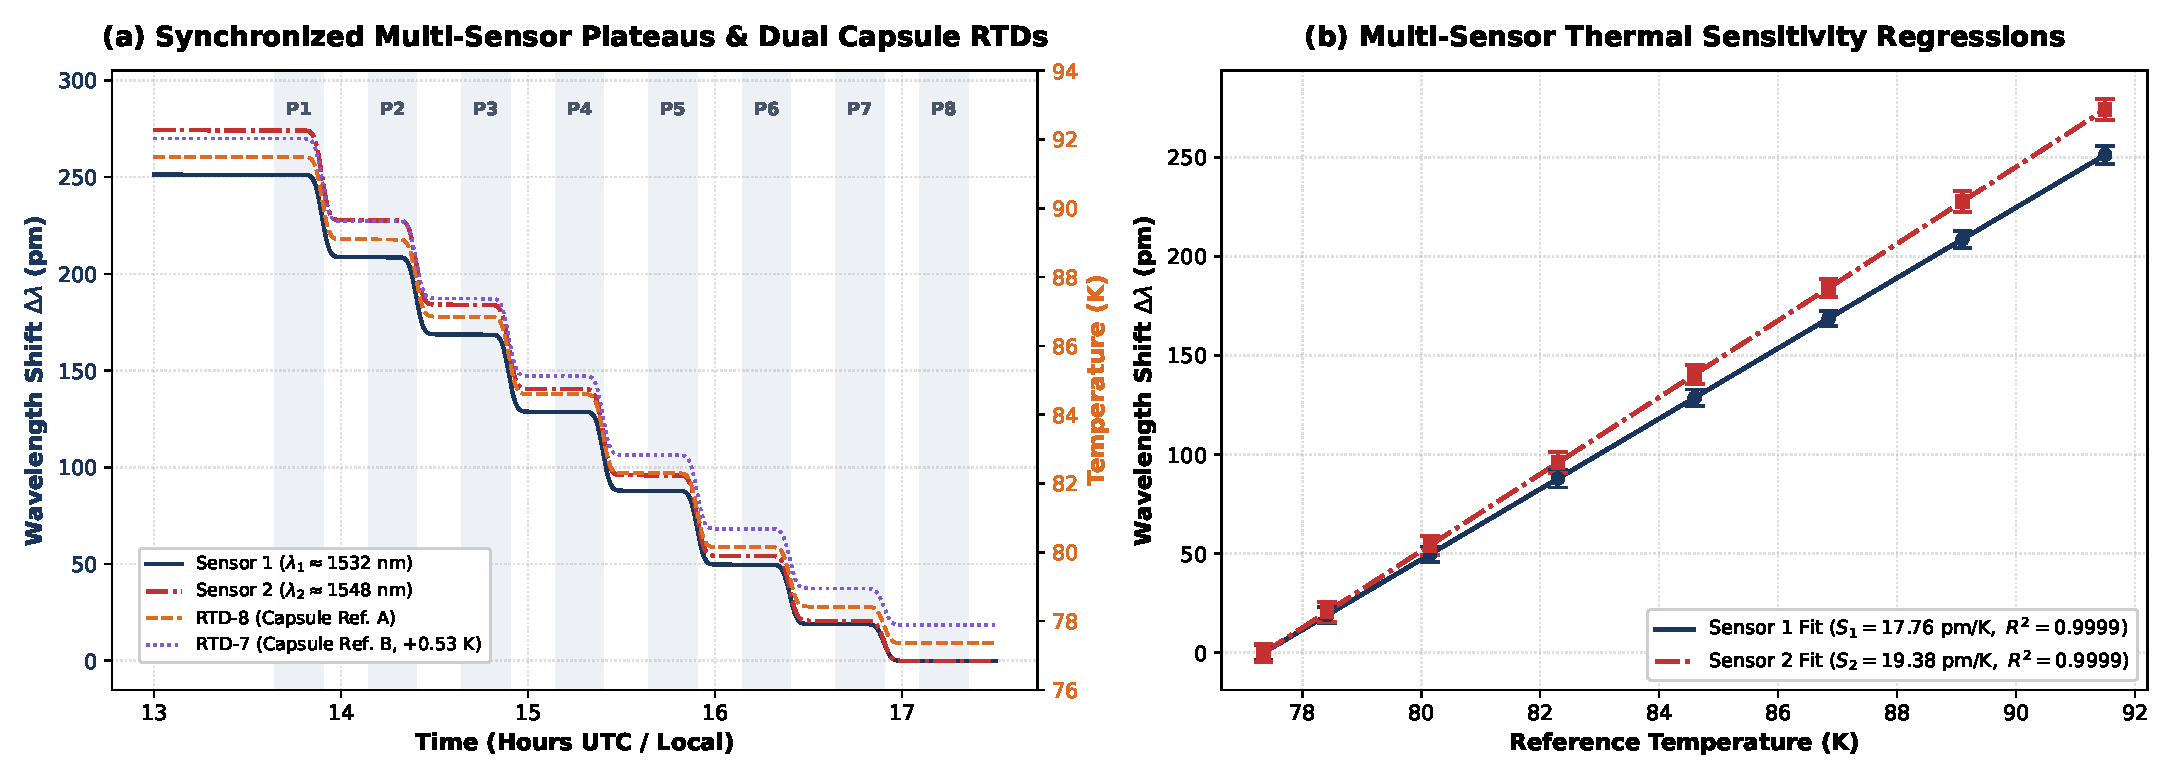
\includegraphics[width=\textwidth]{figures/fig1_peek4_control_plot.pdf}
    \caption{Representative single-run thermal sensitivity calibration for the dual-sensor PEEK-4 fiber ($400\,\mu\text{m}$ jacket diameter) during stepped vessel depressurization (09-06-2026). \textbf{(a)} Synchronized time series across eight steady-state saturation plateaus (P1--P8, shaded green bands), displaying the two multiplexed FBG wavelengths ($\lambda_1 \approx 1532\,\text{nm}$ and $\lambda_2 \approx 1548\,\text{nm}$) alongside the two reference RTDs (RTD-8 and RTD-7) housed in diametrically opposed slots of the cylindrical support within the immersion capsule. The systematic intra-capsule thermal offset of $\Delta T \approx 0.53\,\text{K}$ between RTD-7 and RTD-8 reflects their physical placement relative to residual vertical and circumferential thermal gradients within the liquid bath. \textbf{(b)} Linear regression of the plateau-averaged Bragg wavelength shifts as a function of the reference temperature (RTD-8), yielding $S_1 = 17.76 \pm 0.04\,\text{pm/K}$ ($R^2 = 0.9999$) and $S_2 = 19.38 \pm 0.08\,\text{pm/K}$ ($R^2 = 0.9999$).}
    \label{fig:control_plot_run1}
\end{figure}

As shown in Figure~\ref{fig:control_plot_run1}(a), both optical sensors closely track the stepped depressurization over eight distinct equilibrium plateaus (P1--P8). Simultaneously recorded signals from the two reference RTDs housed in diametrically opposed slots of the cylindrical support within the capsule reveal a stationary thermal offset of $\Delta T = T_{\text{RTD-7}} - T_{\text{RTD-8}} \approx +0.53~\text{K}$. Because this spatial offset remains constant throughout the entire steady-state sequence ($\sigma_{\Delta T} < 15~\text{mK}$ across all plateaus), calibrating either optical grating against RTD-7 versus RTD-8 produces identical sensitivity slopes within $<0.001~\text{pm/K}$, shifting only the absolute intercept. Consequently, the observed difference between Sensor~1 ($17.76 \pm 0.04~\text{pm/K}$) and Sensor~2 ($19.38 \pm 0.08~\text{pm/K}$) represents an intrinsic inter-sensor coating responsivity variation along the fiber length ($\Delta S = 1.62~\text{pm/K}$), rather than an experimental measurement artifact. Both gratings exhibit near-perfect linear responsivity ($R^2 \ge 0.9999$), as summarized in Table~\ref{tab:peek4_run1_summary}.

\begin{table}[htpb]
    \centering
    \small
    \caption{Single-run sensitivity and linearity parameters for the dual-sensor PEEK-4 fiber array (Run 1, 09-06-2026).}
    \label{tab:peek4_run1_summary}
    \begin{tabular}{lccc}
        \toprule
        \textbf{Sensor} & \textbf{Nominal $\lambda_B$ (nm)} & \textbf{Sensitivity $S$ (pm/K)} & $\boldsymbol{R^2}$ \\
        \midrule
        Sensor 1 & $1532.5$ & $17.76 \pm 0.04$ & 0.9999 \\
        Sensor 2 & $1548.8$ & $19.38 \pm 0.08$ & 0.9999 \\
        \bottomrule
    \end{tabular}
\end{table}

To evaluate thermal cycling endurance and long-term calibration fidelity, multi-run repeatability was assessed by subjecting the fibers to three independent cryogenic cooldown and depressurization cycles ($n = 3$) carried out over separate experimental days. Figure~\ref{fig:peek4_repeatability} displays the run-to-run sensitivity evolution for the PEEK-4 fiber. Both multiplexed sensors exhibit outstanding operational stability, with individual run-to-run variations constrained to $\sigma_{\text{rep}} \le 0.45~\text{pm/K}$ and the fiber-averaged ensemble sensitivity remaining within $18.90 \pm 0.29~\text{pm/K}$. Crucially, the relative sensitivity hierarchy between Sensor~1 and Sensor~2 is strictly preserved across all thermal cycles, demonstrating that the polymer-to-cladding interfacial adhesion does not degrade upon cryogenic cycling.

\begin{figure}[htpb]
    \centering
    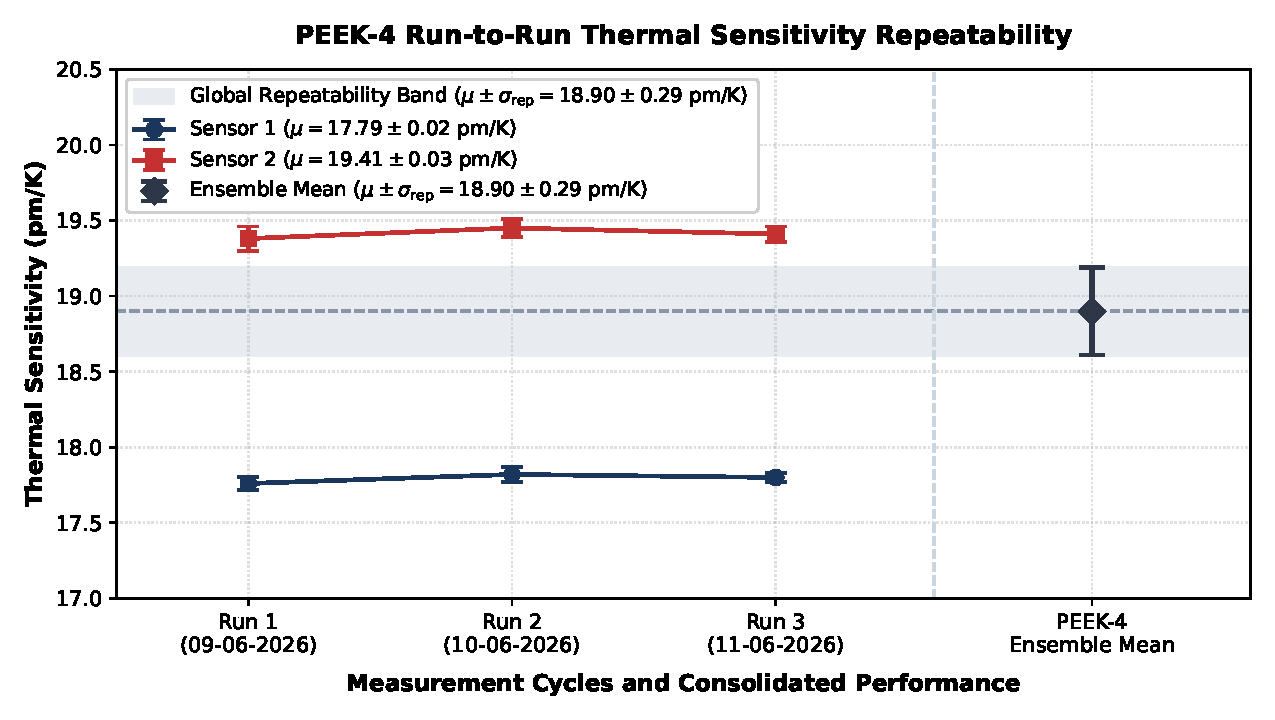
\includegraphics[width=0.88\textwidth]{figures/fig2_peek4_repeatability.pdf}
    \caption{Cryogenic thermal cycling repeatability for the dual-sensor PEEK-4 fiber over three independent experimental runs ($n = 3$). Individual markers represent the sensitivity slopes for Sensor~1 (circles) and Sensor~2 (squares), with vertical error bars indicating individual fit uncertainties ($u_{\text{fit}}$). The ensemble mean sensitivity across all runs and sensors is $\bar{S} = 18.90\,\text{pm/K}$, with the shaded horizontal band designating the global temporal repeatability uncertainty ($\pm 1\sigma_{\text{rep}} = \pm 0.29\,\text{pm/K}$).}
    \label{fig:peek4_repeatability}
\end{figure}

The comprehensive metrological performance across all tested polymeric coatings is consolidated in Table~\ref{tab:repeatability_summary}. Three key metrological metrics are reported:
\begin{enumerate}
    \item \textit{Ensemble Mean Sensitivity} ($\bar{S} \pm \text{SEM}$): The overall average sensitivity and associated standard error of the mean across all gratings and thermal cycles for each coating configuration.
    \item \textit{Worst-Case Repeatability} ($\sigma_{\text{rep}}^{\max}$): The maximum run-to-run standard deviation observed for an individual sensor, quantifying temporal stability under thermal cycling.
    \item \textit{Array Uniformity} ($\sigma_{\text{unif}}$): The inter-sensor standard deviation along a single multi-sensor fiber, reflecting longitudinal fabrication consistency of the polymeric jacket.
\end{enumerate}

\begin{table}[htpb]
    \centering
    \small
    \setlength{\tabcolsep}{4.5pt}
    \caption{Thermal sensitivity, cycling repeatability, and array uniformity across tested fiber coating configurations over three independent experimental runs ($n = 3$).}
    \label{tab:repeatability_summary}
    \begin{tabular}{lcccccc}
        \toprule
        \textbf{Fiber ID} & \textbf{Coating} & \textbf{Diameter} & \textbf{Sensors} & \textbf{Mean Sens. $\bar{S}$} & \textbf{Max Repeat.} & \textbf{Uniformity} \\
        & & ($\mu\text{m}$) & ($M$) & (pm/K) & $\sigma_{\text{rep}}^{\max}$ (pm/K) & $\sigma_{\text{unif}}$ (pm/K) \\
        \midrule
        PEEK-1  & PEEK      & 450 & 1 & $20.59 \pm 0.11$ & 0.19 & --- \\
        PEEK-7  & PEEK      & 450 & 3 & $19.62 \pm 0.32$ & 0.59 & 0.67 \\
        PEEK-4  & PEEK      & 400 & 2 & $18.90 \pm 0.35$ & 0.45 & 0.95 \\
        PEEK-3  & PEEK      & 200 & 1 & $3.12 \pm 0.02$  & 0.04 & --- \\
        FBGS-2  & Ormocer   & 200 & 2 & $7.22 \pm 0.06$  & 0.26 & 0.10 \\
        DW-3    & Ormocer-T & 250 & 2 & $4.71 \pm 0.02$  & 0.04 & 0.06 \\
        POLY-2  & Polyimide & 200 & 2 & $3.64 \pm 0.02$  & 0.07 & 0.01 \\
        \bottomrule
    \end{tabular}
\end{table}

\begin{figure}[htpb]
    \centering
    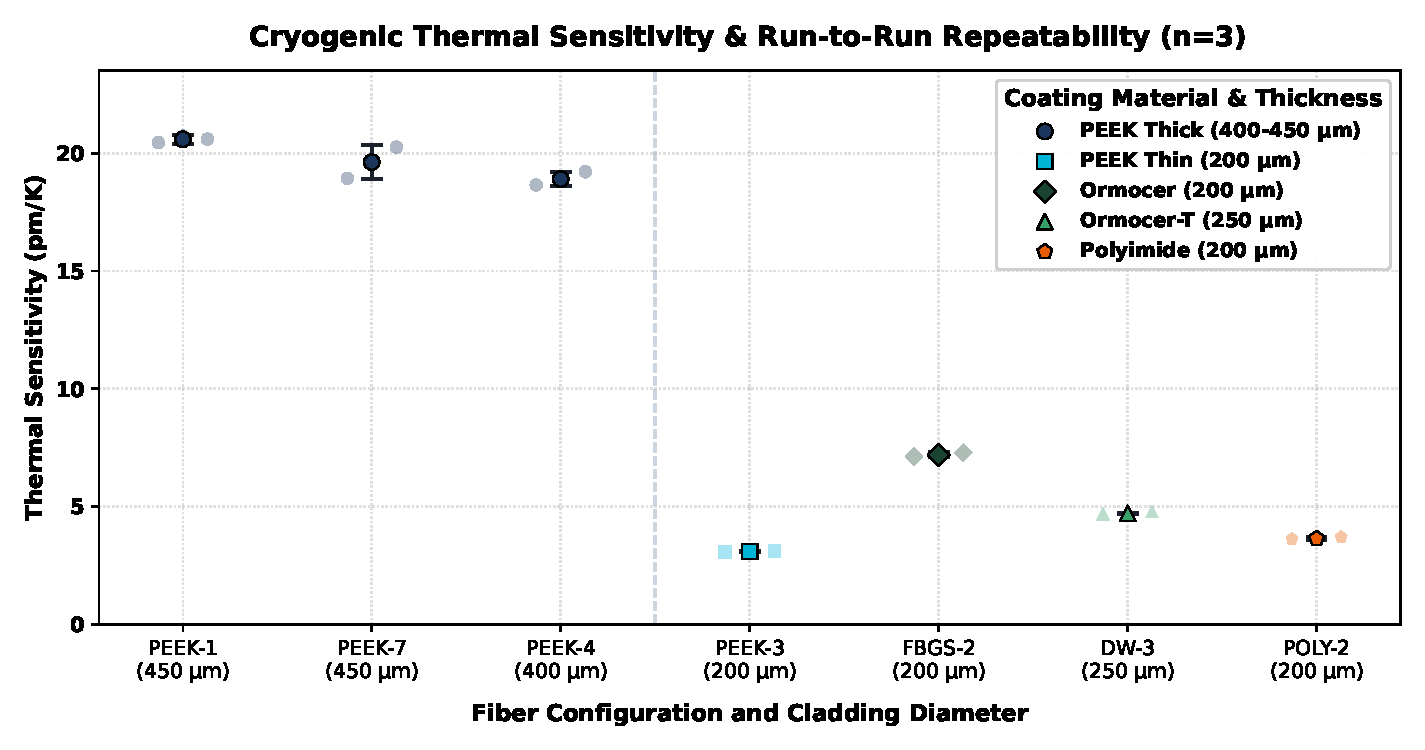
\includegraphics[width=0.88\textwidth]{figures/fig3_global_sensitivity_summary.pdf}
    \caption{Global cryogenic thermal sensitivity comparison across all tested fiber configurations. Bar heights represent the ensemble mean sensitivity ($\bar{S}$), with error bars indicating the run-to-run repeatability standard deviation ($\pm 1\sigma_{\text{rep}}$). Individual cycle measurements are overlaid as jittered markers to depict the experimental distribution across the three independent runs.}
    \label{fig:global_sensitivity_summary}
\end{figure}

% -------------------------------------------------------------------------
\subsubsection{Discussion: Coating Material and Geometric Influences}
% -------------------------------------------------------------------------

The comparative performance consolidated in Table~\ref{tab:repeatability_summary} and Figure~\ref{fig:global_sensitivity_summary} highlights the dominant physical mechanisms governing cryogenic FBG responsivity and stability:

\begin{enumerate}
    \item \textbf{Coating thickness dependency in PEEK fibers:} At liquid nitrogen temperatures ($77$--$93~\text{K}$), the normalized thermo-optic coefficient of fused silica collapses by nearly an order of magnitude, causing the intrinsic thermal sensitivity of bare silica gratings to drop below $1.3~\text{pm/K}$~\cite{Lupi2008,Salin2008,Rajan2013}. The measured thermal response is therefore governed almost exclusively by the axial compressive strain transferred from the contracting polymer sheath due to the thermal expansion coefficient (CTE) mismatch~\cite{Rajan2013,NIST_CryoMaterials}. Comparing the PEEK configurations demonstrates the critical impact of jacket geometry: thick thermoplastic jackets ($\varnothing\,400$--$450\,\mu\text{m}$, represented by PEEK-1, PEEK-4, and PEEK-7) consistently yield large cryogenic sensitivities ranging between $18.90$ and $20.59~\text{pm/K}$—an enhancement of more than $\times 15$ over bare silica. In contrast, the thin PEEK-3 fiber ($\varnothing\,200\,\mu\text{m}$) achieves only $3.12 \pm 0.02~\text{pm/K}$. The substantial cross-sectional area of the $400$--$450\,\mu\text{m}$ jackets ($A_{\text{jacket}}/A_{\text{silica}} \approx 9$--$12$) provides the necessary mechanical rigidity to overcome the elastic counter-straining of the silica core, whereas the $200~\mu\text{m}$ jacket lacks sufficient cross-section to compress the stiff glass core effectively.

    \item \textbf{Material properties and strain transfer fidelity:} For fibers of identical outer diameter ($\sim 200\,\mu\text{m}$), the thermal responsivity is dictated by the intrinsic cryogenic CTE and the interfacial shear strength of the primary coating~\cite{Zhao2007,NIST_CryoMaterials}. Ormocer-coated fibers (FBGS-2, $7.22 \pm 0.06~\text{pm/K}$) and Ormocer-T (DW-3, $4.71 \pm 0.02~\text{pm/K}$) substantially outperform standard polyimide (POLY-2, $3.64 \pm 0.02~\text{pm/K}$). Furthermore, both draw-tower Ormocer and Ormocer-T coatings exhibit outstanding intra-fiber uniformity ($\sigma_{\text{unif}} \le 0.10~\text{pm/K}$) and thermal cycling repeatability ($\sigma_{\text{rep}}^{\max} \le 0.06~\text{pm/K}$), reflecting superior interfacial adhesion and homogeneous radial curing during fiber drawing characteristic of hybrid inorganic-organic networks~\cite{Popall1998}.

    \item \textbf{Thermal cycling stability and fabrication uniformity:} Across all tested configurations, the relative sensitivity rankings and absolute values remained highly repeatable across the three independent cooldown cycles ($300~\text{K} \leftrightarrow 77~\text{K}$). The thick PEEK fibers exhibited moderate inter-sensor variations ($\sigma_{\text{unif}} \approx 0.67$--$0.95~\text{pm/K}$), which is characteristic of the melt-extrusion process used for thick thermoplastic sleeving. Nevertheless, their individual temporal stability ($\sigma_{\text{rep}} \le 0.45~\text{pm/K}$) confirms that repeated deep cryogenic immersion does not induce micro-cracking, delamination, or degradation of the mechanical strain coupling.
\end{enumerate}

%-------------------------------
\subsection{FBG sensitivity to milli-kelvin temperature changes (Vicky)}
\label{subsec:milli_kelvin}

% Placeholder for next section

% ==========================================
\section{Conclusions (?)}
% ==========================================
\begin{itemize}
    \item Summary of the most repeatable coating materials 
    \item Summary of the best coating and thickness (PEEK 400 (20 pm/K)).
    \item Viability of the manual pressure-based plateau method.
    \item Future work improvements (new pressure set-up).
\end{itemize}

The repeatability study demonstrates the feasibility of the manual pressure-based setup for characterizing FBG sensors at cryogenic temperatures. Based on our findings, the PEEK-coated fibers, particularly the $400~\mu$m variant, exhibit the highest thermal sensitivity, making them ideal for high-precision applications. Conversely, Ormocer coatings offer superior temporal response, suitable for fast transient measurements. \\

Table~\ref{tab:conclusion_matrix} provides a summary recommendation for material selection based on the specific requirements of the cryogenic system.

\begin{table}[htpb]
    \centering
    \caption{Performance matrix for coating selection in cryogenic applications.}
    \label{tab:conclusion_matrix}
    \begin{tabular}{lcccc}
        \toprule
        \textbf{Coating} & \textbf{Sensitivity} & \textbf{Repeatability} & \textbf{Thermal Lag} & \textbf{Best for...} \\
        \midrule
        Ormocer-T & Moderate & Excellent & Low & General purpose \\
        PEEK ($400~\mu m$) & High & Good & High & Precision mapping \\
        Polyimide & Low & High & Very Low & Dynamic changes \\
        \bottomrule
    \end{tabular}
\end{table}

% ==========================================
% References
% ==========================================
\begin{thebibliography}{99}

\bibitem{Othonos1997}
A. Othonos, 
``Fiber Bragg gratings, 
\textit{Review of Scientific Instruments}, vol. 68, no. 12, pp. 4309--4341, 1997.

\bibitem{Rao1997}
Y. J. Rao, 
``In-fibre Bragg grating sensors, 
\textit{Measurement Science and Technology}, vol. 8, no. 4, pp. 355--375, 1997.

\bibitem{Kashyap2009}
R. Kashyap, 
\textit{Fiber Bragg Gratings}, 2nd ed. San Diego: Academic Press, 2009.

\bibitem{James2002}
S. W. James and R. P. Tatam, 
``Optical fibre long-period grating sensors: characteristics and application, 
\textit{Measurement Science and Technology}, vol. 14, no. 5, R49, 2003.

\bibitem{Lupi2008}
C. Lupi, F. Felli, L. Ippoliti, et al., 
``Metal coating for enhancing the sensitivity of fibre Bragg grating sensors at cryogenic temperatures, 
\textit{Smart Materials and Structures}, vol. 17, no. 3, 035005, 2008.

\bibitem{Salin2008}
M. Salin et al.,
``Fiber Bragg grating sensors for cryogenic temperature measurements, 
\textit{Proceedings of SPIE - The International Society for Optical Engineering}, 2008.

\bibitem{Bock2004}
W. J. Bock, M. Beaulieu, S. E. Kreismanis, and W. Urbanczyk, 
``Pressure effects on fiber Bragg grating temperature sensors, 
\textit{IEEE Transactions on Instrumentation and Measurement}, vol. 53, no. 4, pp. 1107--1112, 2004.

\bibitem{Zhao2007}
Y. Zhao et al.,
``Performance analysis of polyimide-coated fiber Bragg grating sensors,
\textit{Optics and Lasers in Engineering}, vol. 45, no. 10, pp. 1011--1015, 2007.

\bibitem{Rajan2013}
G. Rajan, B. Gangadhara Prusty, and K. S. C. Kuang,
``Polymer-coated fiber Bragg grating sensors for cryogenic temperature sensing,
\textit{IEEE Sensors Journal}, vol. 13, no. 5, pp. 1928--1933, 2013.

\bibitem{NIST_CryoMaterials}
E. D. Marquardt, J. P. Le, and R. D. Radebaugh,
``Cryogenic material properties database,
in \textit{Proceedings of the 11th International Cryocooler Conference}, Keystone, CO, pp. 681--687, 2000.

\bibitem{Popall1998}
M. Popall et al.,
``ORMOCERs---inorganic-organic hybrid materials for photonic packaging,
\textit{Microelectronics Reliability}, vol. 38, no. 12, pp. 1941--1946, 1998.

\bibitem{Bao2007}
X. Bao and L. Chen, 
``Recent progress in distributed fiber optic sensors, 
\textit{Sensors}, vol. 7, no. 12, pp. 3095--3125, 2007.

\bibitem{LabVIEW2023}
National Instruments, LabVIEW 2023 Help: Data Acquisition Fundamentals, Austin, TX, 2023.

\bibitem{FemtoSenseManual}
FemtoSense, ``Optical Interrogator Model: Technical Data Sheet and User Manual,.

\bibitem{Acciarri2020ProtoDUNE}
B. Abi et al. (DUNE Collaboration),
``First results on ProtoDUNE-SP liquid argon time projection chamber performance from a beam run at the CERN Neutrino Platform,
\textit{Journal of Instrumentation}, vol. 15, no. 12, P12004, 2020.

\bibitem{RTDs_paper}
M. Antonova, J. Capó, A. Cervera, P. Fernández, M.Á. García-Peris, X. Pons,
Millikelvin-precision temperature sensing for advanced cryogenic detectors,
Nuclear Instruments and Methods in Physics Research Section A: Accelerators, Spectrometers, Detectors and Associated Equipment,
Volume 1082, Part 2,
2026,
171062,
ISSN 0168-9002,
https://doi.org/10.1016/j.nima.2025.171062.

\bibitem{Edejer1967}
M. P. Edejer and G. Thodos,
``Vapor pressures of normal saturated fluids from the triple point to the critical point,
\textit{Journal of Chemical and Engineering Data}, vol. 12, no. 2, pp. 206--209, 1967.

\bibitem{Lemmon2025NIST}
E. W. Lemmon, I. H. Bell, M. L. Huber, and M. O. McLinden,
\textit{NIST Standard Reference Database 23: Reference Fluid Thermodynamic and
Transport Properties -- REFPROP, Version 10.0},
National Institute of Standards and Technology, 2018.
Available: \url{https://www.nist.gov/srd/refprop}

\end{thebibliography}

\end{document}
